\chapter{Interfejs użytkownika - TODO}
\label{cha:UI}
W niniejszym rozdziale skupię się na szczegółowym opisie interfejsu użytkownika. Zostaną przedstawione najważniejsze funkcję, które pomogą użytkownikowi w korzystaniu z programu. Omówinone zostaną poszczególne warstwy wyświetlone na mapie, przełączanie między nimi oraz tworzenie własnych warst, przedstawiających dodaną przez użytkownika informację. W pierwszej sekcji przedstawiony zostanie widok główny aplikacji wraz z dokładnym omówieniem. W dalszych częsciach tego rozdziału, opisane zostaną kolejne warstwy. Na końcu przedstawiony zostanie sposób, jak dodawać własne obiekty, żeby były widoczne na mapie.
\newpage
\section{Widok główny aplikacji}
\label{sec:mainView}

Rys. \ref{mainView}. przedstawia widok główny aplikacji. W lewym górnym rogu znajdują się dwa przyciski: ''+'' oraz ''-''. Umożliwiają one przybliżanie i oddalanie widoku mapy. W prawym górnym rogu znajduję się menu wyboru wyświetlanej warstwy. Szczegóły dostępne w rozdziale \ref{sec:layerMenu}. Ponadto, użytkownik posiada możliwość, za pomocą myszki, przesuwania obecnie wyświetlanej mapy w dowolnym kierunku. Mapa pobierana jest w czasie rzeczywistym ze strony OpenStreetMap.

\begin{figure}[h]
\caption{Widok główny aplikacji}
\label{mainView}
\centering
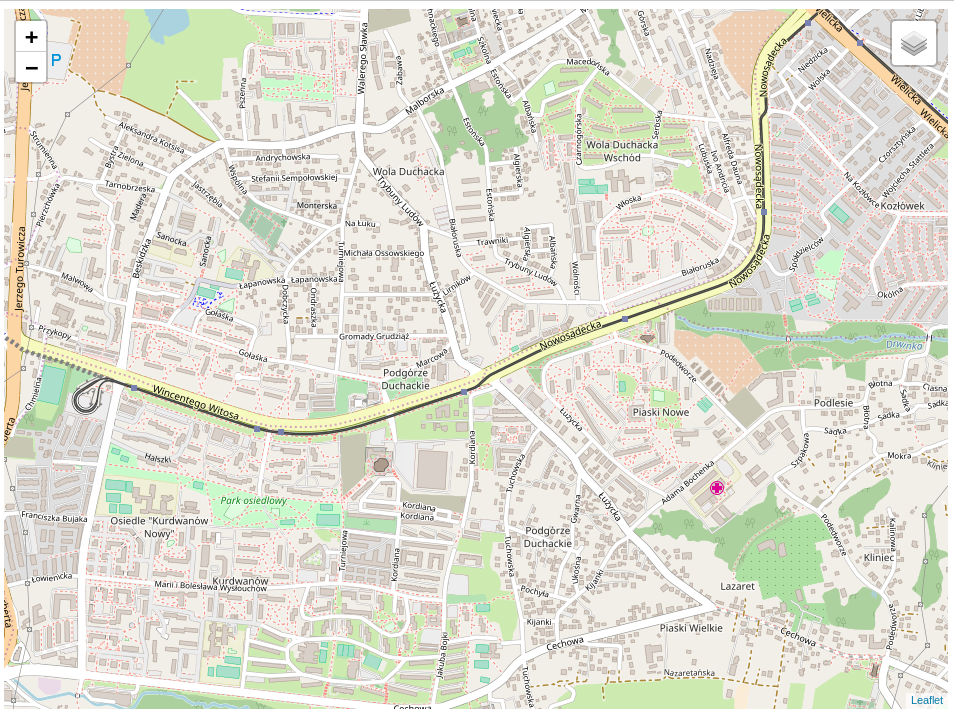
\includegraphics[width=1.1\textwidth]{mainScreen}
\end{figure}

\newpage

\section{Menu wyboru warstw}
\label{sec:layerMenu}

Rys. \ref{sec:mainLayerView}. przedstawia menu wyboru warstw. Dostępny jest dopiero po najechaniu kursorem myszki. Umozliwia wyświetlanie na mapie elementów, które użytkownik w danej chwili potrzebuje. 

\begin{figure}[h]
\caption{Menu wyboru warstw}
\label{sec:mainLayerView}
\centering
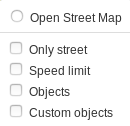
\includegraphics[width=0.4\textwidth]{layerMenu}
\end{figure}

Menu wyboru warst, Rys. \ref{sec:mainLayerView}, składa się z pięciu elementów:
\begin{itemize}
\item \textbf{Open Street Map} - domyślna warstwa, służąca do wyświetlania głównej mapy.
\item \textbf{Only street} - służy do zaznaczania na mapie, wszystkich dostępnych ulic. Więcej szczegółów znajduje się w rozdziale \ref{sec:onlyStreet}
\item \textbf{Speed limit} - najważniejsza warstwa, przedstawiajaca dopuszczalne prędkości na drogach. Więcej szczegółów znajduje się w rozdziale \ref{sec:speedLimit}
\item \textbf{Objects} - wyświetla obiekty istotne dla algorytmu obliczajacego predkość pojazdów. W ich skład wchodzą np. przystanki autobusowe i tramwajowe, szkoły, kościoły, place zabaw itp. Więcej szczegółów znajduje się w rozdziale \ref{sec:objects}
\item \textbf{Custom objects} - wyświetla dane wprowadzone przez wszystkich użytkowników aplikacji. Więcej szczegółów znajduje się w rozdziale \ref{sec:customObjects}
\end{itemize}

Istotną funkcjonalnością jest możliwość wyświetlania dowolnych kombinacji warstw. Użytkownik może zaznaczyć dowolną liczbę widoków, które zostaną wyswietlone na głównej mapie.

\newpage
\section{Widok zaznaczonych ulic}
\label{sec:onlyStreet}

Rys. \ref{sec:onlyStreetMap} przedstawia mapę, na której zaznaczone są poszczególne odcinki dróg. Reprezentowane są przez niebieskie linie łamane, przebiegającą przez sam jej środek. Zostały uzglednione różnego rodzaju klasy dróg, takie jak: 
\begin{itemize}
\item autostrady
\item drogi ekspresowe
\item drogi główne ruchu przyspieszonego
\item drogi główne
\item drogi zbiorcze
\item drogi lokalne
\item drogi dojazdowe
\end{itemize}

\begin{figure}[h]
\caption{Widok zaznaczonych ulic}
\label{sec:onlyStreetMap}
\centering
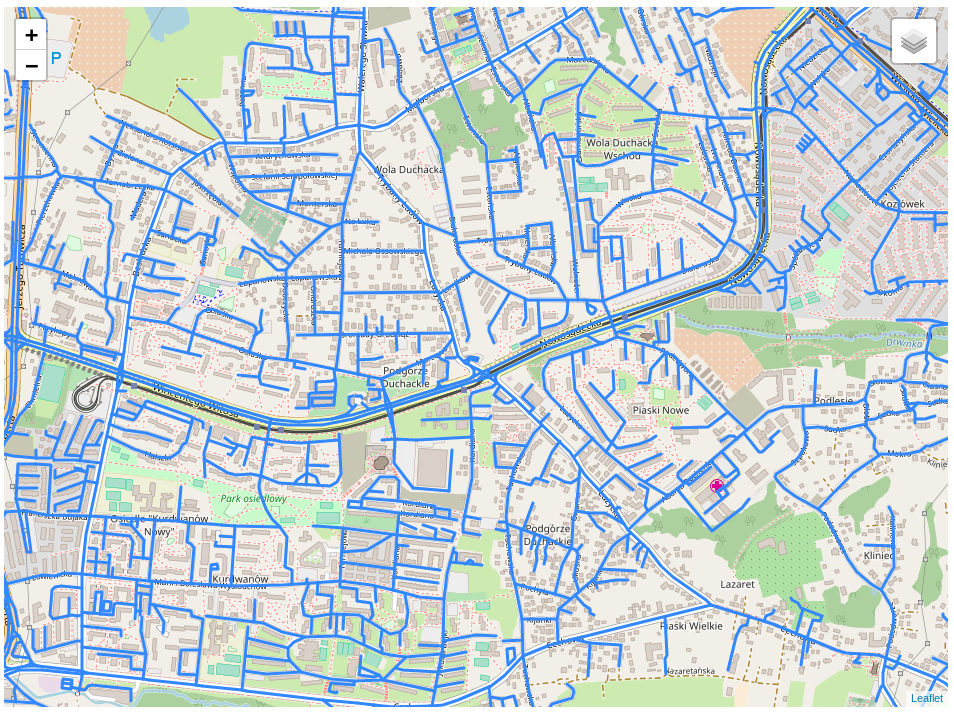
\includegraphics[width=1.03\textwidth]{onlyStreet}
\end{figure}

\newpage
\section{Widok dopuszczalnych ograniczeń prędkości}
\label{sec:speedLimit}


Na mapie z Rys. \ref{sec:speedLimitMap}, zostały umieszczone ograniczenia prędkości dla każdego odcinka drogi. Do wyznaczania tych ograniczeń, algorytm uwzględnił szereg czynników, które zostały opisane w późniejszych rozdziałach. Dla lepszej wizualizacji wyznaczonych danych, do wykonania Rys. \ref{sec:speedLimitMap}., został włączony także widok zaznaczonych ulic, opisany w rozdziale \ref{sec:onlyStreet}.

\begin{figure}[h]
\caption{Widok dopuszczalnych ograniczeń prędkości}
\label{sec:speedLimitMap}
\centering
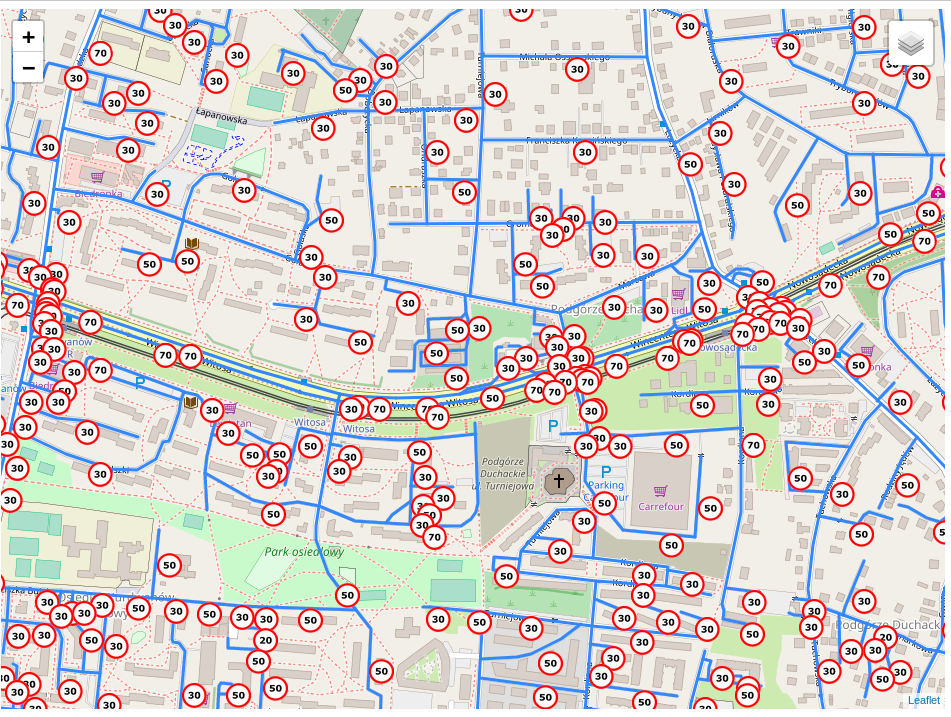
\includegraphics[width=1.03\textwidth]{speedLimit}
\end{figure}

\newpage
\section{Widok istotnych obiektów pobranych z OSM}
\label{sec:objects}

Rys. \ref{sec:objectsMap} przedstawia istotne, z puktu widzenia algorytmu, obiekty pobrane z OpenStreetMap. W ich skład wchodzą:
\begin{itemize}
\item przedszkola i szkoły
\item przystanki autobusowe i tramwajowe
\item przejścia dla pieszczych
\item sklepy i miejsca kultu religijnego
\item place zabaw
\end{itemize}

\begin{figure}[h]
\caption{Widok istotnych obiektów pobranych z OSM}
\label{sec:objectsMap}
\centering
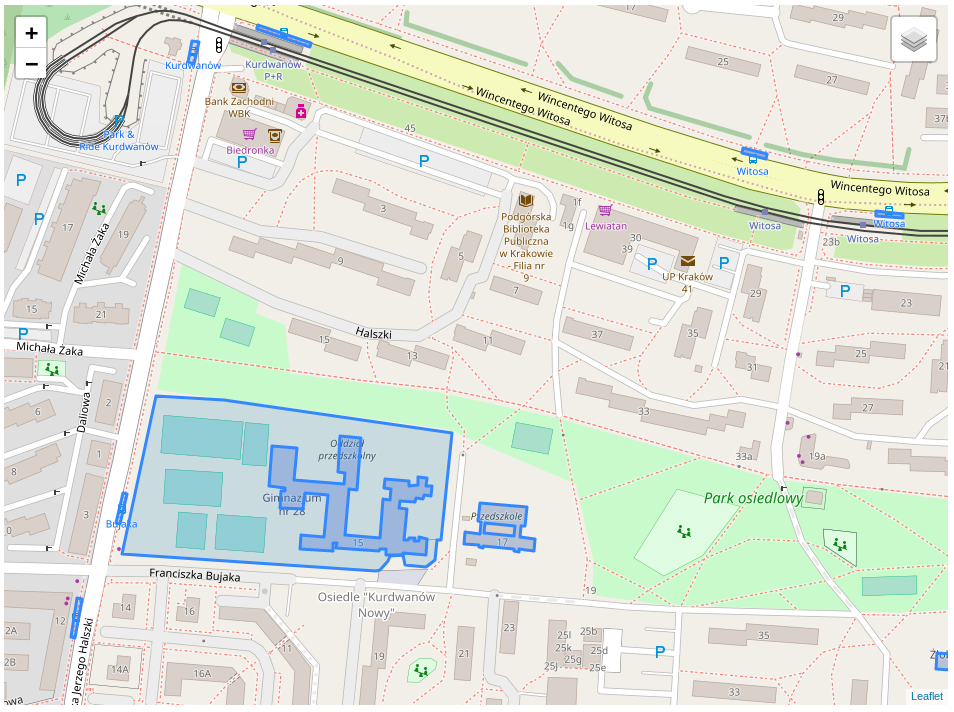
\includegraphics[width=1.03\textwidth]{objects}
\end{figure}

\newpage
\section{Widok obiektów zdefiniowanych przez użytkownika}
\label{sec:customObjects}

\newpage
\section{Dodawanie własnych obiektów}
\label{sec:addedCustomObjects}